%%----------------------------------------------------------------------------
%% Presentatie HoGent Bedrijf en Organisatie
%%----------------------------------------------------------------------------
%% Auteur: Bert Van Vreckem [bert.vanvreckem@hogent.be]

\documentclass{beamer}

%==============================================================================
% Aanloop
%==============================================================================

%---------- Packages ----------------------------------------------------------

\usepackage{graphicx,multicol}
\usepackage{comment,enumerate,hyperref}
\usepackage{amsmath,amsfonts,amssymb}
\usepackage{tikz}
\usepackage[dutch]{babel}
\usepackage[utf8]{inputenc}
\usepackage{multirow}
\usepackage{eurosym}
\usepackage{listings}
\usepackage[T1]{fontenc}
\usepackage{lmodern}
\usepackage{textcomp}
\usepackage{framed}
\usepackage{wrapfig}

%---------- Configuratie ------------------------------------------------------

\usetikzlibrary{arrows,shapes,backgrounds,positioning,shadows}

\usetheme{hogent}

%---------- Commando-definities -----------------------------------------------

\newcommand{\tabitem}{~~\llap{\textbullet}~~}

%---------- Info over de presentatie ------------------------------------------

\title[Intro]{Native Apps 1: Hello Android}
\author{Karine Samyn, Jens Buysse}
\date{AJ 2017-2018}

%==============================================================================
% Inhoud presentatie
%==============================================================================

\begin{document}

%---------- Front matter ------------------------------------------------------

% Dia met het HoGent logo
\HoGentLogo

% Titeldia met faculteitslogo
\titleframe

%---------- Inhoud ------------------------------------------------------------

\begin{frame}
  \frametitle{Inhoud}

  \tableofcontents
\end{frame}

%---------- Back matter -------------------------------------------------------

\section{Overzicht cursus}

\sectionframe{}

\begin{frame}{Doelstellingen}
\begin{itemize}
	\item Kan een grafische user interface volgens de richtlijnen gedefinieerd door de stijlgids van Android ontwikkelen en verantwoorden.
\item	Kan gebruik maken van de meest courante APIs binnen het Android platform en het gebruik ervan verantwoorden. 
\item	Kan de courante technieken en designpatronen binnen Android gebruiken en het gebruik ervan verantwoorden. 
\item	Kan een bestaande webservice aanspreken in Android en het gebruik ervan verantwoorden. 
\item	Kan een kwaliteitsvolle mobiele Android applicatie ontwerpen, ontwikkelen, documenteren en testen 
\end{itemize}
	
\end{frame}

\begin{frame}{Inhoud}
\begin{itemize}
	\item Hello Android
	\item	Activities
	\item	User Interfaces : layouts en action bar
	\item Fragments 
	\item	Intents and Broadcastreceivers
	\item RecyclerView and CardViews
	\item  Persistency: Shared Preferences en Activity State
	\item  Persistency en SQLite
	\item Netwerk en Services
	\item Testing
\end{itemize}

\end{frame}

\begin{frame}{Onderwijsvorm}
\begin{itemize}
	\item Flipped Classroom (combinatie online/face-to-face)
	\item Oefeningen
	\begin{itemize}
	\item Thuis verder afwerken
	\item Indienen op GIT. Bij elke oef een git classroom link
	\item Wordt bevraagd op het examen
\end{itemize}

	\item Cursusmateriaal
	\begin{itemize}
		\item De cursus: https://github.com/eothein/nativeapps1
		\item M. Reto, Professional Android Development. 2017.
		\item 	M. L. Murphy, The Busy Coder’s Guide to Android Development. https://commonsware.com/Android/,2017, vol. CommonsWare.
		
		\item External resources and references Google. (Sep. 2017). Android developers guide, [Online]. Available: https://developer.android.com/guide/platform/index.html.
		
	\end{itemize}
\end{itemize}

\end{frame}

\begin{frame}{Examen}
\begin{itemize}
	\item Mondeling examen – GESLOTEN BOEK
	\begin{itemize}
	\item Theoretisch luik 
	\item Praktisch luik (op eigen laptop)
	\begin{itemize}
	\item Vragen over de oefeningen (eigen code, geen gedeelde code) op github classroom waarin wordt nagegaan of je de doelstellingen hebt bereikt 
	\item Alle oefeningen moet je gemaakt hebben. Als je een vraag krijgt over een oefening die je niet gemaakt heb -> 0
	\item Je mag samenwerken voor de oefeningen, MAAR schrijf de code zelf!\\
		\end{itemize}
		\end{itemize}
		\end{itemize}
\end{frame}


\section{Hello Android}
\sectionframe{}

\begin{frame}{Wat installeren}
\begin{itemize}

	\item JDK 1.8
	\item Android Studio version 2.3.3 or later, installeert ook de Android SDK\break \url{https://developer.android.com/studio/install.html}
		\end{itemize}	

\end{frame}
\begin{frame}{Open Source Android}
\begin{itemize}
	
	\item 2005: Android inc
	\item 2008: Android 1.0 en HTC Dream
	\item Open Handset Alliance
	\item Maar is Android  open source?
\end{itemize}	

\end{frame}
\begin{frame}{Android versies }
\begin{figure}[ht]
	\centering
	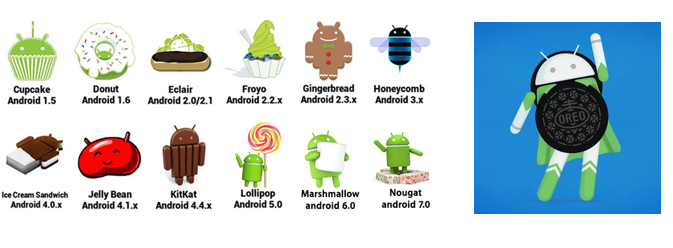
\includegraphics[width=\textwidth]{img/hello/android_versies.png}
	\label{fig:android versies}
	\caption{De verschillende android versies}
\end{figure}	
\end{frame}

\begin{frame}{Android versies/API levels }
\begin{figure}[ht]
	\centering
	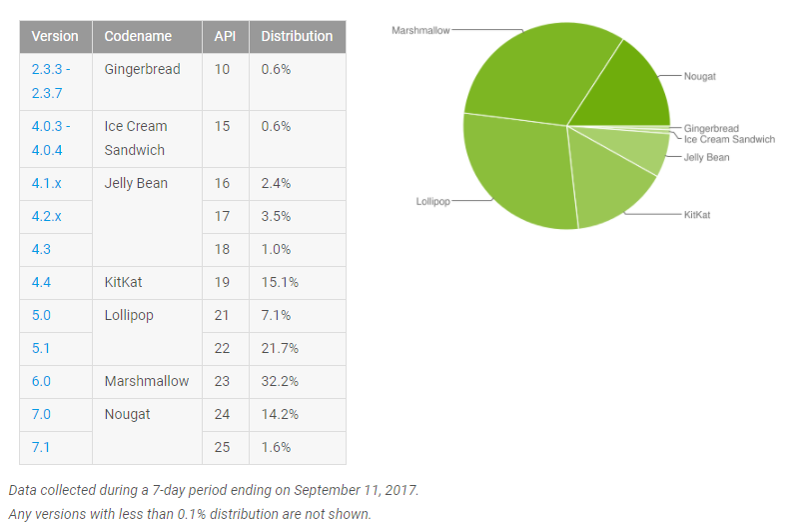
\includegraphics[width=\textwidth]{img/hello/api_levels.png}
	\label{fig:apilevels}
	\caption{Keuze van Android platform en API level}
\end{figure}
Meer info op \url{https://developer.android.com/about/dashboards/index.html
}	
\end{frame}

\begin{frame}{De Android software stack }
\begin{figure}[ht]
	\centering
	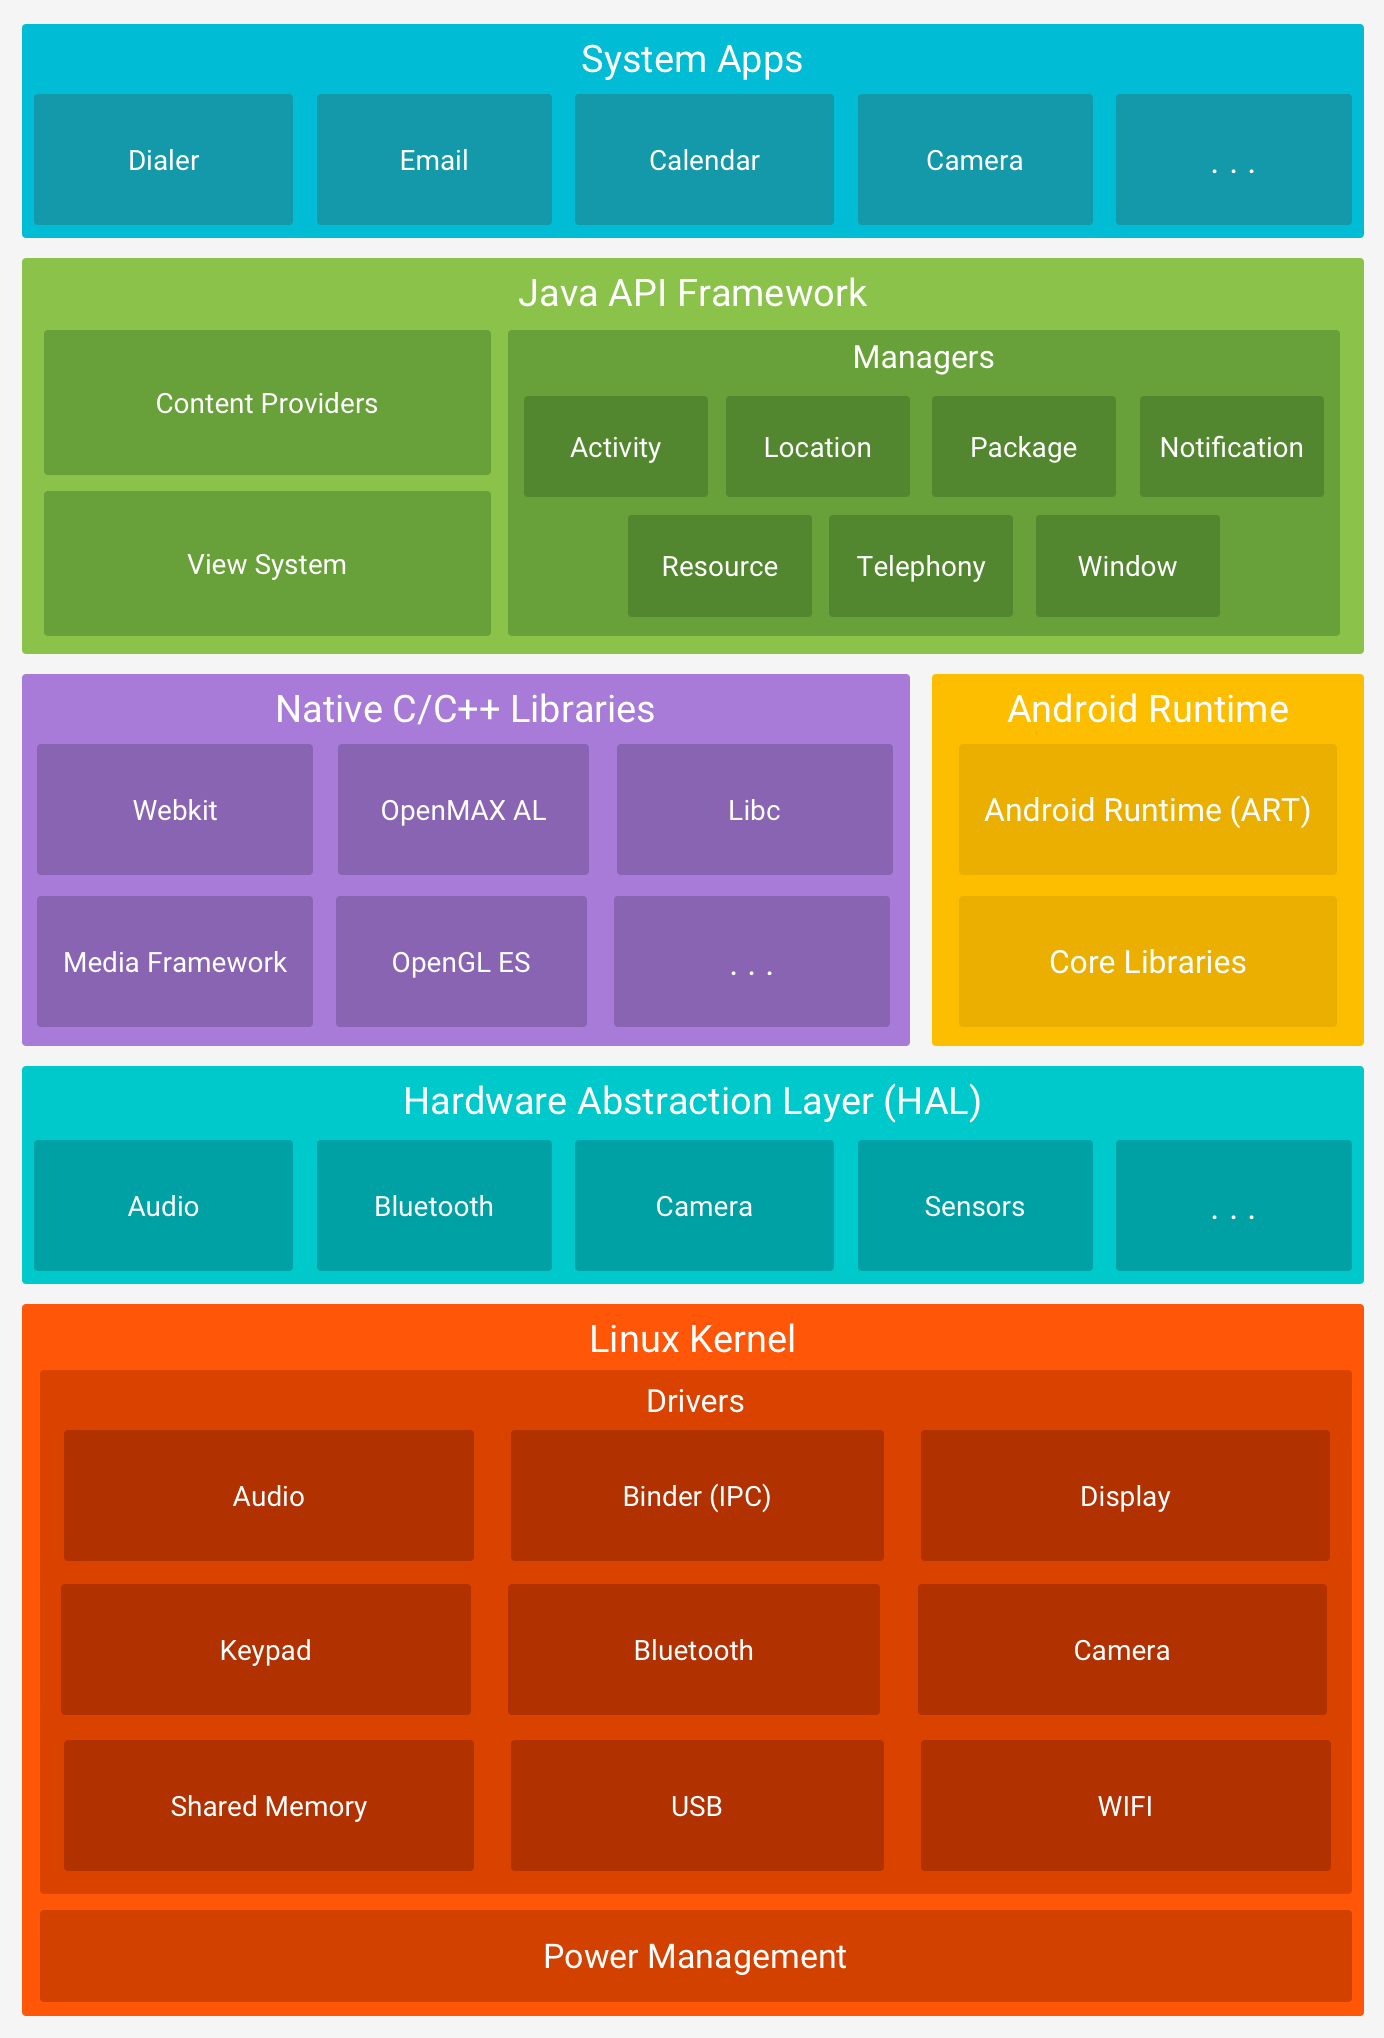
\includegraphics[height=\textheight]{img/hello/android-stack.png}
	\label{fig:stack}
	\caption{Android is an open source, Linux-based software stack created for a wide array of devices and form factors. The following diagram shows the major components of the Android platform.}
\end{figure}	
\end{frame}

\begin{frame}{De Android software stack }
\begin{itemize}	
	\item De Android runtime
\end{itemize}
\begin{figure}[ht]
	\centering
	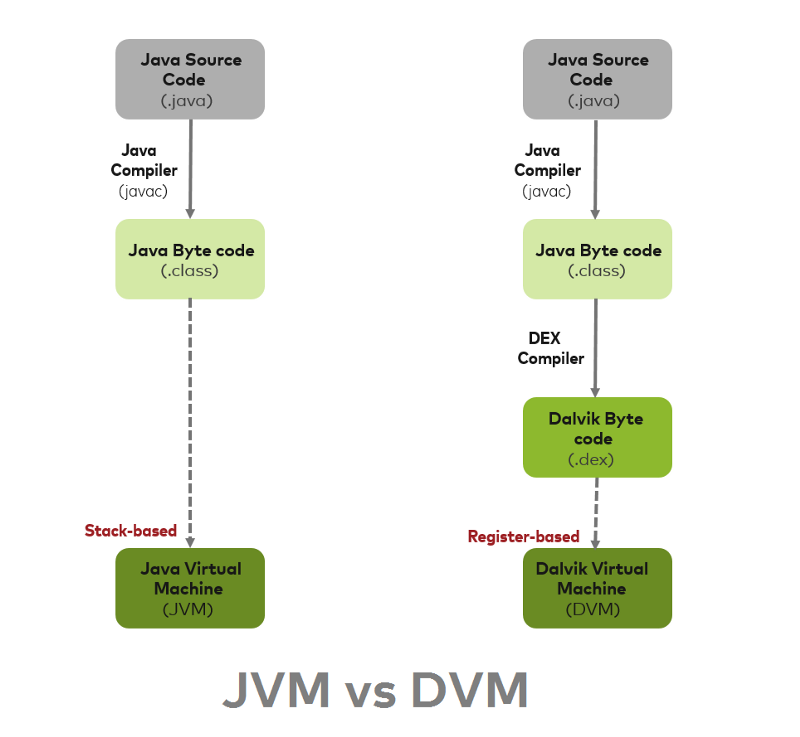
\includegraphics[height=\textheight]{img/hello/jvmdvm.png}
	\label{fig:jvm versus dvm}
	\caption{JVM versus DVM. Figure from https://android.jlelse.eu/closer-look-at-android-runtime-dvm-vs-art-1dc5240c3924}
\end{figure}	
\end{frame}

\begin{frame}{De Android software stack }
\begin{itemize}	
	\item De Android runtime
\end{itemize}
\begin{figure}[ht]
	\centering
	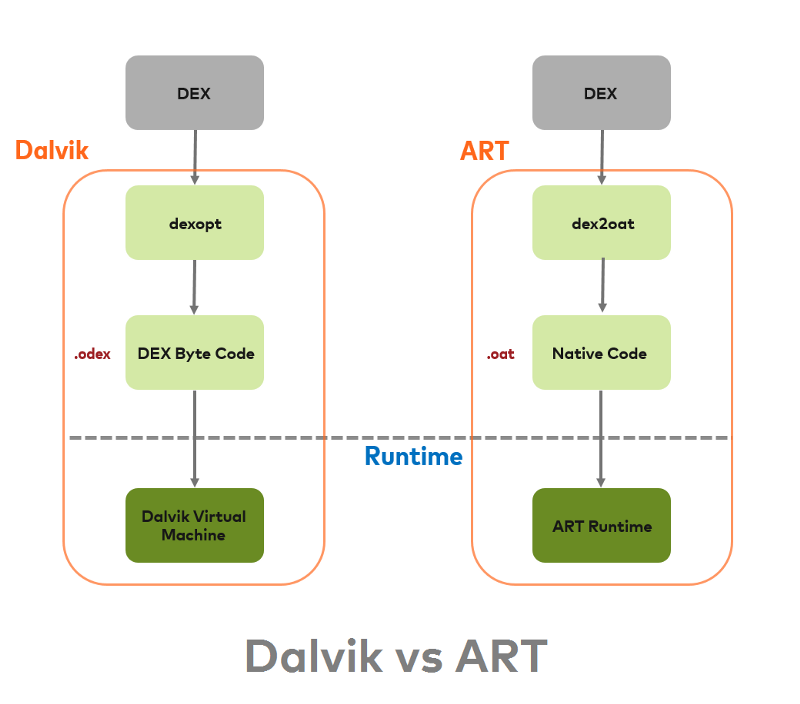
\includegraphics[width=\textwidth]{img/hello/dalvikART.png}
	\label{fig:Dalvik versus ART}
	\caption{Dalvik versus ART. Figure from https://android.jlelse.eu/closer-look-at-android-runtime-dvm-vs-art-1dc5240c3924}
\end{figure}	
\end{frame}


\section{Lab}
\sectionframe{}

\begin{frame}{Lab}

	In dit lab bouwen we een eenvoudig Android project en runnen we de app.
	

		Volg de tutorial \url{https://developer.android.com/training/basics/firstapp/index.html}

	

\end{frame}
\begin{frame}[fragile]{Het build proces}

	\begin{figure}[hb]
		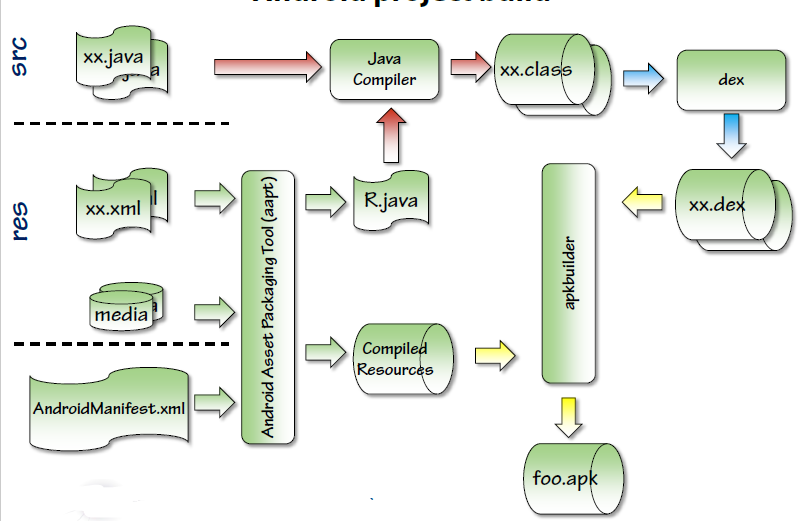
\includegraphics[width=\textwidth]{img/hello/buildproces.png}
		\label{fig:develop}
		\caption{The flow for building an Android application. }
	\end{figure}

\end{frame}





\end{document}
